\chapter{General Context of the Project}
\section{Introduction}
This chapter presents the overall context of the project, highlighting the
company \textbf{Smart Automation Technologies} and introducing its objectives
and challenges. We will examine the problem statement, the objectives, the
adopted approaches, and the expected results. Furthermore, we will detail the
organization of the project, including the chosen methodology and the planned
schedule.   

\section{Presentation of the Company}
\textbf{Smart Automation Technologies (SAT)} was founded by a group of senior
consultants specializing in new information technologies, data science, and
artificial intelligence. The company is distinguished by its commitment to
innovation and performance, offering its expertise to businesses and public
administrations seeking tailored solutions to their needs and constraints.  

SAT’s approach is based on continuous research and constant development in order
to remain at the forefront of information technology and artificial
intelligence. As a trusted partner, the company supports its clients from the
design to the evolution of their information systems, as well as in their needs
for studies, training, and integrated software solutions. The company’s main
objective is to establish long term relationships with its clients, acting as an
essential link in their value chain.  

By providing strong expertise in computing and machine learning, SAT enables its
clients to focus on their core business activities while relying on advanced and
reliable technological solutions.  

\begin{figure}[H]
    \centering
    
\includegraphics[width=0.5\textwidth]{images/logo.jpeg}
    \caption{Company Logo}
\end{figure}




\subsection{Approaches and Values}
\textbf{SMART AUTOMATION TECHNOLOGIES} adopts a
differentiation oriented approach by placing great importance on ethics and
professional management. This approach ensures a transparent and committed
relationship with its clients, based on trust and mutual understanding.  

The company fosters close relationships with its clients in order to better
understand their needs and anticipate their expectations. This relationship is
based on trust and open communication, thus promoting fruitful and sustainable
collaboration.  

Furthermore, \textbf{SMART AUTOMATION TECHNOLOGIES} recognizes the value
of its human capital and invests in the development of its employees. They
benefit from guidance, monitoring, evaluation, and continuous training,
thereby ensuring a high level of competence and commitment.


\begin{figure}[H]
    \centering
    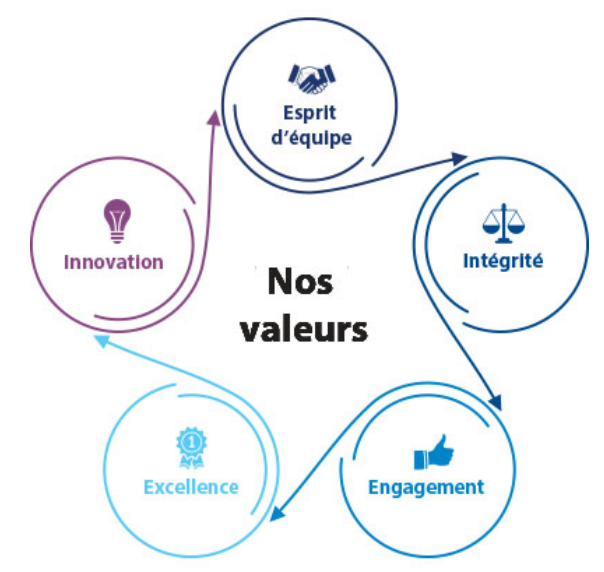
\includegraphics[width=0.5\textwidth]{images/values.png}
    \caption{Values of SAT}
\end{figure}

\subsection{Business Areas and Services}
\textbf{SMART AUTOMATION TECHNOLOGIES} offers a comprehensive range
of dedicated services and solutions, leveraging its experience and expertise
to meet the diverse needs of its clients.  
Below is an overview of the business areas and services provided:  

\begin{itemize}
    \item \textbf{Dedicated Services and Solutions:}  
    \textbf{SMART AUTOMATION TECHNOLOGIES} applies its know-how in the
    design and implementation of information systems tailored to each client.  
    These dedicated solutions are designed to deliver real added value across
    various sectors of activity.
     \item \textbf{Support and Training:}  
    In addition to its design services, \textbf{SMART AUTOMATION TECHNOLOGIES}
    provides continuous support to its clients, as well as training to ensure the
    optimal use of the implemented solutions.
\end{itemize}
The consulting strategy of \textbf{SMART AUTOMATION TECHNOLOGIES} is based on
a client, project, and method centered approach. The company supports its clients
in their organizational and development projects, guiding their evolution strategy
towards an information system orientation and transformation plan.  
Here are some of the specific operations carried out by
\textbf{SMART AUTOMATION TECHNOLOGIES}:  

\begin{itemize}
    \item IT Governance and Project Management
    \item Development of an IT Master Plan
    \item Information System Urbanization
    \item Project Ownership Assistance
    \item Software Architecture
    \item Turnkey Solutions
    \item Software Benchmarking and Audit
\end{itemize}

These business areas and services illustrate the commitment of
\textbf{SMART AUTOMATION TECHNOLOGIES} to delivering personalized and
innovative solutions while supporting its clients in their digital and strategic
transformation.

\subsection{Products and Solutions}
\textbf{SMART AUTOMATION TECHNOLOGIES} is committed to creating
products that address real world needs, with a strong focus on the integration
of artificial intelligence, data science, and Big Data particularly in the
fields of industry, logistics, marketing, and finance.  

The company is also exploring the implementation of the e-Transformation
process, built around the principle of a digital, intelligent, and decision making
ecosystem.  

\section{Project Overview}
\subsection{Study of the Existing Situation}
\hspace{1em}Before the implementation of the proposed solution, the company did not have
an existing infrastructure dedicated to the collection, storage, or processing of
IoT sensor data.  

The absence of such a platform meant that sensor data, although available, could
not be fully exploited for real-time analysis, predictive maintenance, or decision
support. Without a centralized and automated system, the processing of data
would have required manual interventions, which is neither
scalable nor reliable.  

This lack of an existing solution limited the company’s ability to take advantage
of advanced techniques such as Big Data analytics, streaming data processing, or
artificial intelligence integration. It also created significant barriers to ensuring
data quality, operational efficiency, and the possibility of anticipating failures
through predictive models.  

Accordingly, the specific challenges that our solutions aim to address include:  

\begin{enumerate}
    \item \textbf{Massive Data Management:} The vast amount of data generated by data-driven projects requires an ecosystem capable of storing, processing, and analyzing information in an efficient and scalable manner.  
  
    \item \textbf{Real-Time Processing:} Critical applications such as predictive maintenance and operational decision-making demand rapid and responsive data processing capabilities.  
    \item \textbf{Scalability of Resources:} The ability to scale infrastructure up or down based on workload fluctuations is essential to maintain cost efficiency, performance, and adaptability to business needs.  
\end{enumerate}


\subsection{Proposed Solution}

\hspace{1em}To address the identified challenges, the proposed solution consists of
building a scalable and reliable platform capable of managing large volumes of
IoT sensor data in real time. The platform aims to centralize data flows,
support advanced processing, and provide actionable insights for decision making.  

\hspace{1em}The main objectives of the project are as follows:

\begin{enumerate}
    \item \textbf{Improve data management:} Establish an infrastructure capable of efficiently handling the continuous flow of IoT data while ensuring reliability and scalability.
    \item \textbf{Enable real time analysis:} Provide mechanisms to process and analyze sensor data instantly, supporting timely and accurate decision making.
    \item \textbf{Integrate predictive capabilities:} Incorporate advanced AI models, such as LSTM and GRU, to forecast equipment behavior and enable predictive maintenance strategies.
    \item \textbf{Enrich datasets:} Use generative models, such as GANs, to produce synthetic data that enhances the quality and diversity of available datasets for improved analytics and model training.
    \item \textbf{Ensure long term value:} Store and organize processed and raw data in a way that supports both immediate operations and future analytical needs, ensuring the sustainability of the platform.
\end{enumerate}

\hspace{1em}Through this solution, the company will benefit from a unified platform
capable of transforming raw IoT sensor streams into valuable knowledge,
strengthening predictive maintenance practices and unlocking new opportunities
for data driven innovation.

\subsection{Project Planning and Timeline}
\begin{figure}[h!]
    \centering
    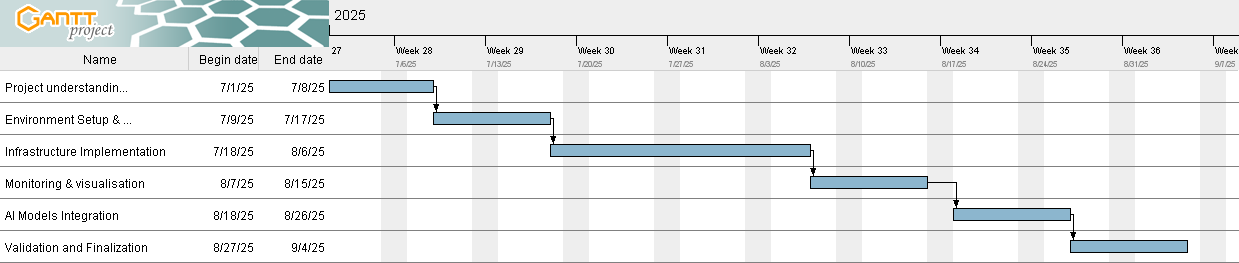
\includegraphics[width=\textwidth]{images/gantt.png}
    \caption{Project Gantt Chart}
\end{figure}

The Gantt chart above illustrates the planning of the project over a two-month
period. It highlights the different phases, starting with project understanding
and environment setup, followed by infrastructure implementation, monitoring
and visualization, integration of AI models, and finally the validation and
finalization phase. This organization ensures a logical progression and balanced
distribution of tasks throughout the project duration.

\section{Conclusion}
The first chapter provided a comprehensive overview of \textbf{Smart Automation
Technologies} and the context in which the IoT platform project is undertaken.
It highlighted the company’s objectives, values, business areas, and solutions,
while identifying key challenges in IoT data management. The proposed solution
and project timeline offer a structured approach to building a scalable, real-time
platform that supports predictive analytics and operational efficiency. This
foundation sets the stage for the state of the art and a detailed technical implementation described
in the following chapters.





